% ============================================================
%  Sistema Multi-Agente para Análisis de Deserción Estudiantil
%  Proyecto Final — Inteligencia Artificial · EAFIT 2026-1
% ============================================================
\documentclass[11pt, a4paper]{article}

\usepackage[spanish]{babel}
\usepackage[utf8]{inputenc}
\usepackage[T1]{fontenc}
\usepackage[top=2cm, bottom=2cm, left=2.5cm, right=2.5cm]{geometry}
\usepackage{parskip}
\setlength{\parskip}{4pt}
\usepackage{graphicx}
\usepackage{booktabs}
\usepackage{tabularx}
\usepackage{float}
\usepackage{caption}
\usepackage[labelfont=bf, font=small]{caption}
\usepackage{subcaption}
\usepackage{amsmath}
\usepackage{hyperref}
\hypersetup{colorlinks=true, linkcolor=black, citecolor=blue, urlcolor=blue}
\usepackage{fancyhdr}
\pagestyle{fancy}
\fancyhf{}
\rhead{\small Deserción Estudiantil · EAFIT 2026-1}
\lhead{\small Sistema Multi-Agente}
\cfoot{\thepage}
\usepackage{tikz}
\usetikzlibrary{shapes.geometric, arrows.meta, positioning}

% ── Título compacto ──────────────────────────────────────────
\title{\textbf{Sistema Multi-Agente para Análisis de Deserción Estudiantil}\\[4pt]
\large Proyecto Final — Inteligencia Artificial · Universidad EAFIT · 2026-1}
\author{
  Juan José Restrepo \quad \href{mailto:jjrestrepc@eafit.edu.co}{\texttt{jjrestrepc@eafit.edu.co}}
  \and
  Samuel Cadavid Zapata \quad \href{mailto:scadavidz@eafit.edu.co}{\texttt{scadavidz@eafit.edu.co}}
}
\date{Mayo 2026}

% ============================================================
\begin{document}
\maketitle
\thispagestyle{fancy}

\begin{abstract}
\noindent
Se presenta un sistema multi-agente para predecir deserción estudiantil universitaria
y generar reportes ejecutivos automáticos. Sobre el dataset UCI de Portugal
($n{=}4{,}424$ estudiantes, 36 variables), se construyó un pipeline que integra
modelado con \textit{machine learning} (Random Forest, AUC-ROC~$=0.9335$,
F1~$=0.7879$) con un sistema de cuatro agentes orquestado en LangGraph
que combina recuperación aumentada por generación (RAG) sobre literatura
científica para producir reportes ejecutivos accionables. El módulo RAG
obtuvo 100\% de exactitud en un conjunto de diez preguntas de evaluación.
\end{abstract}

% ============================================================
\section{Introducción}

La deserción universitaria afecta a más del 40\% de los estudiantes en
América Latina~\cite{tinto1987}, con impacto directo en la sostenibilidad
institucional y el desarrollo profesional de los individuos. La detección
temprana mediante modelos predictivos, combinada con generación automática
de reportes, representa una oportunidad concreta para que las instituciones
actúen de forma preventiva.

Este trabajo responde a la pregunta: \textit{¿Puede un sistema multi-agente
predecir la deserción estudiantil con métricas sólidas y generar reportes
ejecutivos enriquecidos con contexto bibliográfico?} Las contribuciones son:
(1) un pipeline ML reproducible sin \textit{data leakage} con AUC-ROC~$=0.9335$;
(2) cuatro agentes LangGraph bajo patrón \textit{fan-out} paralelo;
(3) un módulo RAG sobre cinco documentos científicos con 100\% de exactitud;
y (4) una aplicación Streamlit que integra todo el sistema.

% ============================================================
\section{Datos y Análisis Exploratorio}

\subsection{Dataset y partición}

Se utilizó el dataset \textit{Predict Students' Dropout and Academic
Success}~\cite{realinho2022} (UCI, id~$=697$): 4{,}424 estudiantes,
36 variables académicas, socioeconómicas y demográficas. La variable
objetivo se binarizó: $y{=}1$ (Dropout) vs.\ $y{=}0$ (Graduate/Enrolled).
La tasa de deserción es 32.1\%, lo que genera desbalance y justifica
el uso de F1 y AUC-ROC como métricas principales (Figura~\ref{fig:dist}).
El dataset se dividió estratificadamente en 70\% entrenamiento (3{,}096),
15\% validación (664) y 15\% test (664), \textbf{antes} de cualquier
transformación para evitar \textit{data leakage}.

\begin{figure}[H]
  \centering
  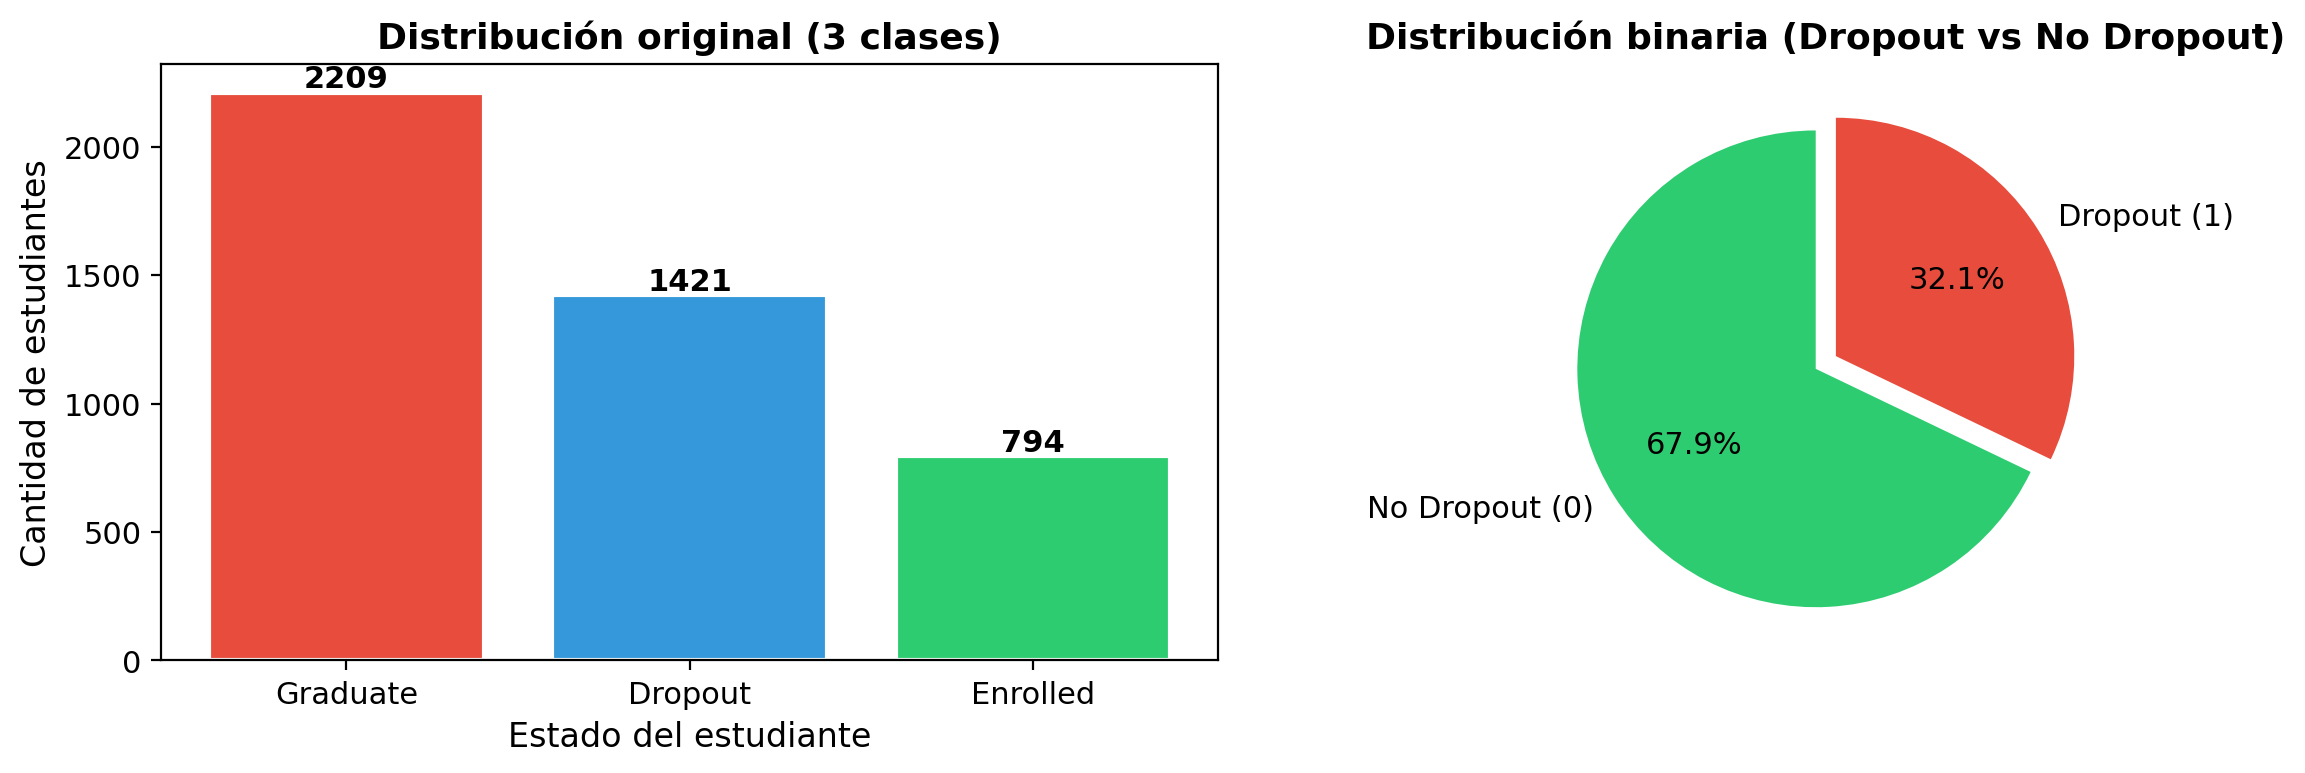
\includegraphics[width=0.82\textwidth]{figures/01_distribucion_objetivo.png}
  \caption{Distribución de la variable objetivo. La clase minoritaria
           (Dropout, 32.1\%) justifica el uso de métricas F1 y AUC-ROC.}
  \label{fig:dist}
\end{figure}

\subsection{Hallazgos principales}

El dataset no presenta valores nulos. El análisis de correlaciones
(Figura~\ref{fig:corr}) confirma que las variables académicas del primer
y segundo semestre —unidades aprobadas y calificaciones— son los predictores
más fuertes. Las variables socioeconómicas (\textit{Tuition fees up to date},
\textit{Debtor}, \textit{Scholarship holder}) actúan como factores de
riesgo secundarios~\cite{delen2010}.

\begin{figure}[H]
  \centering
  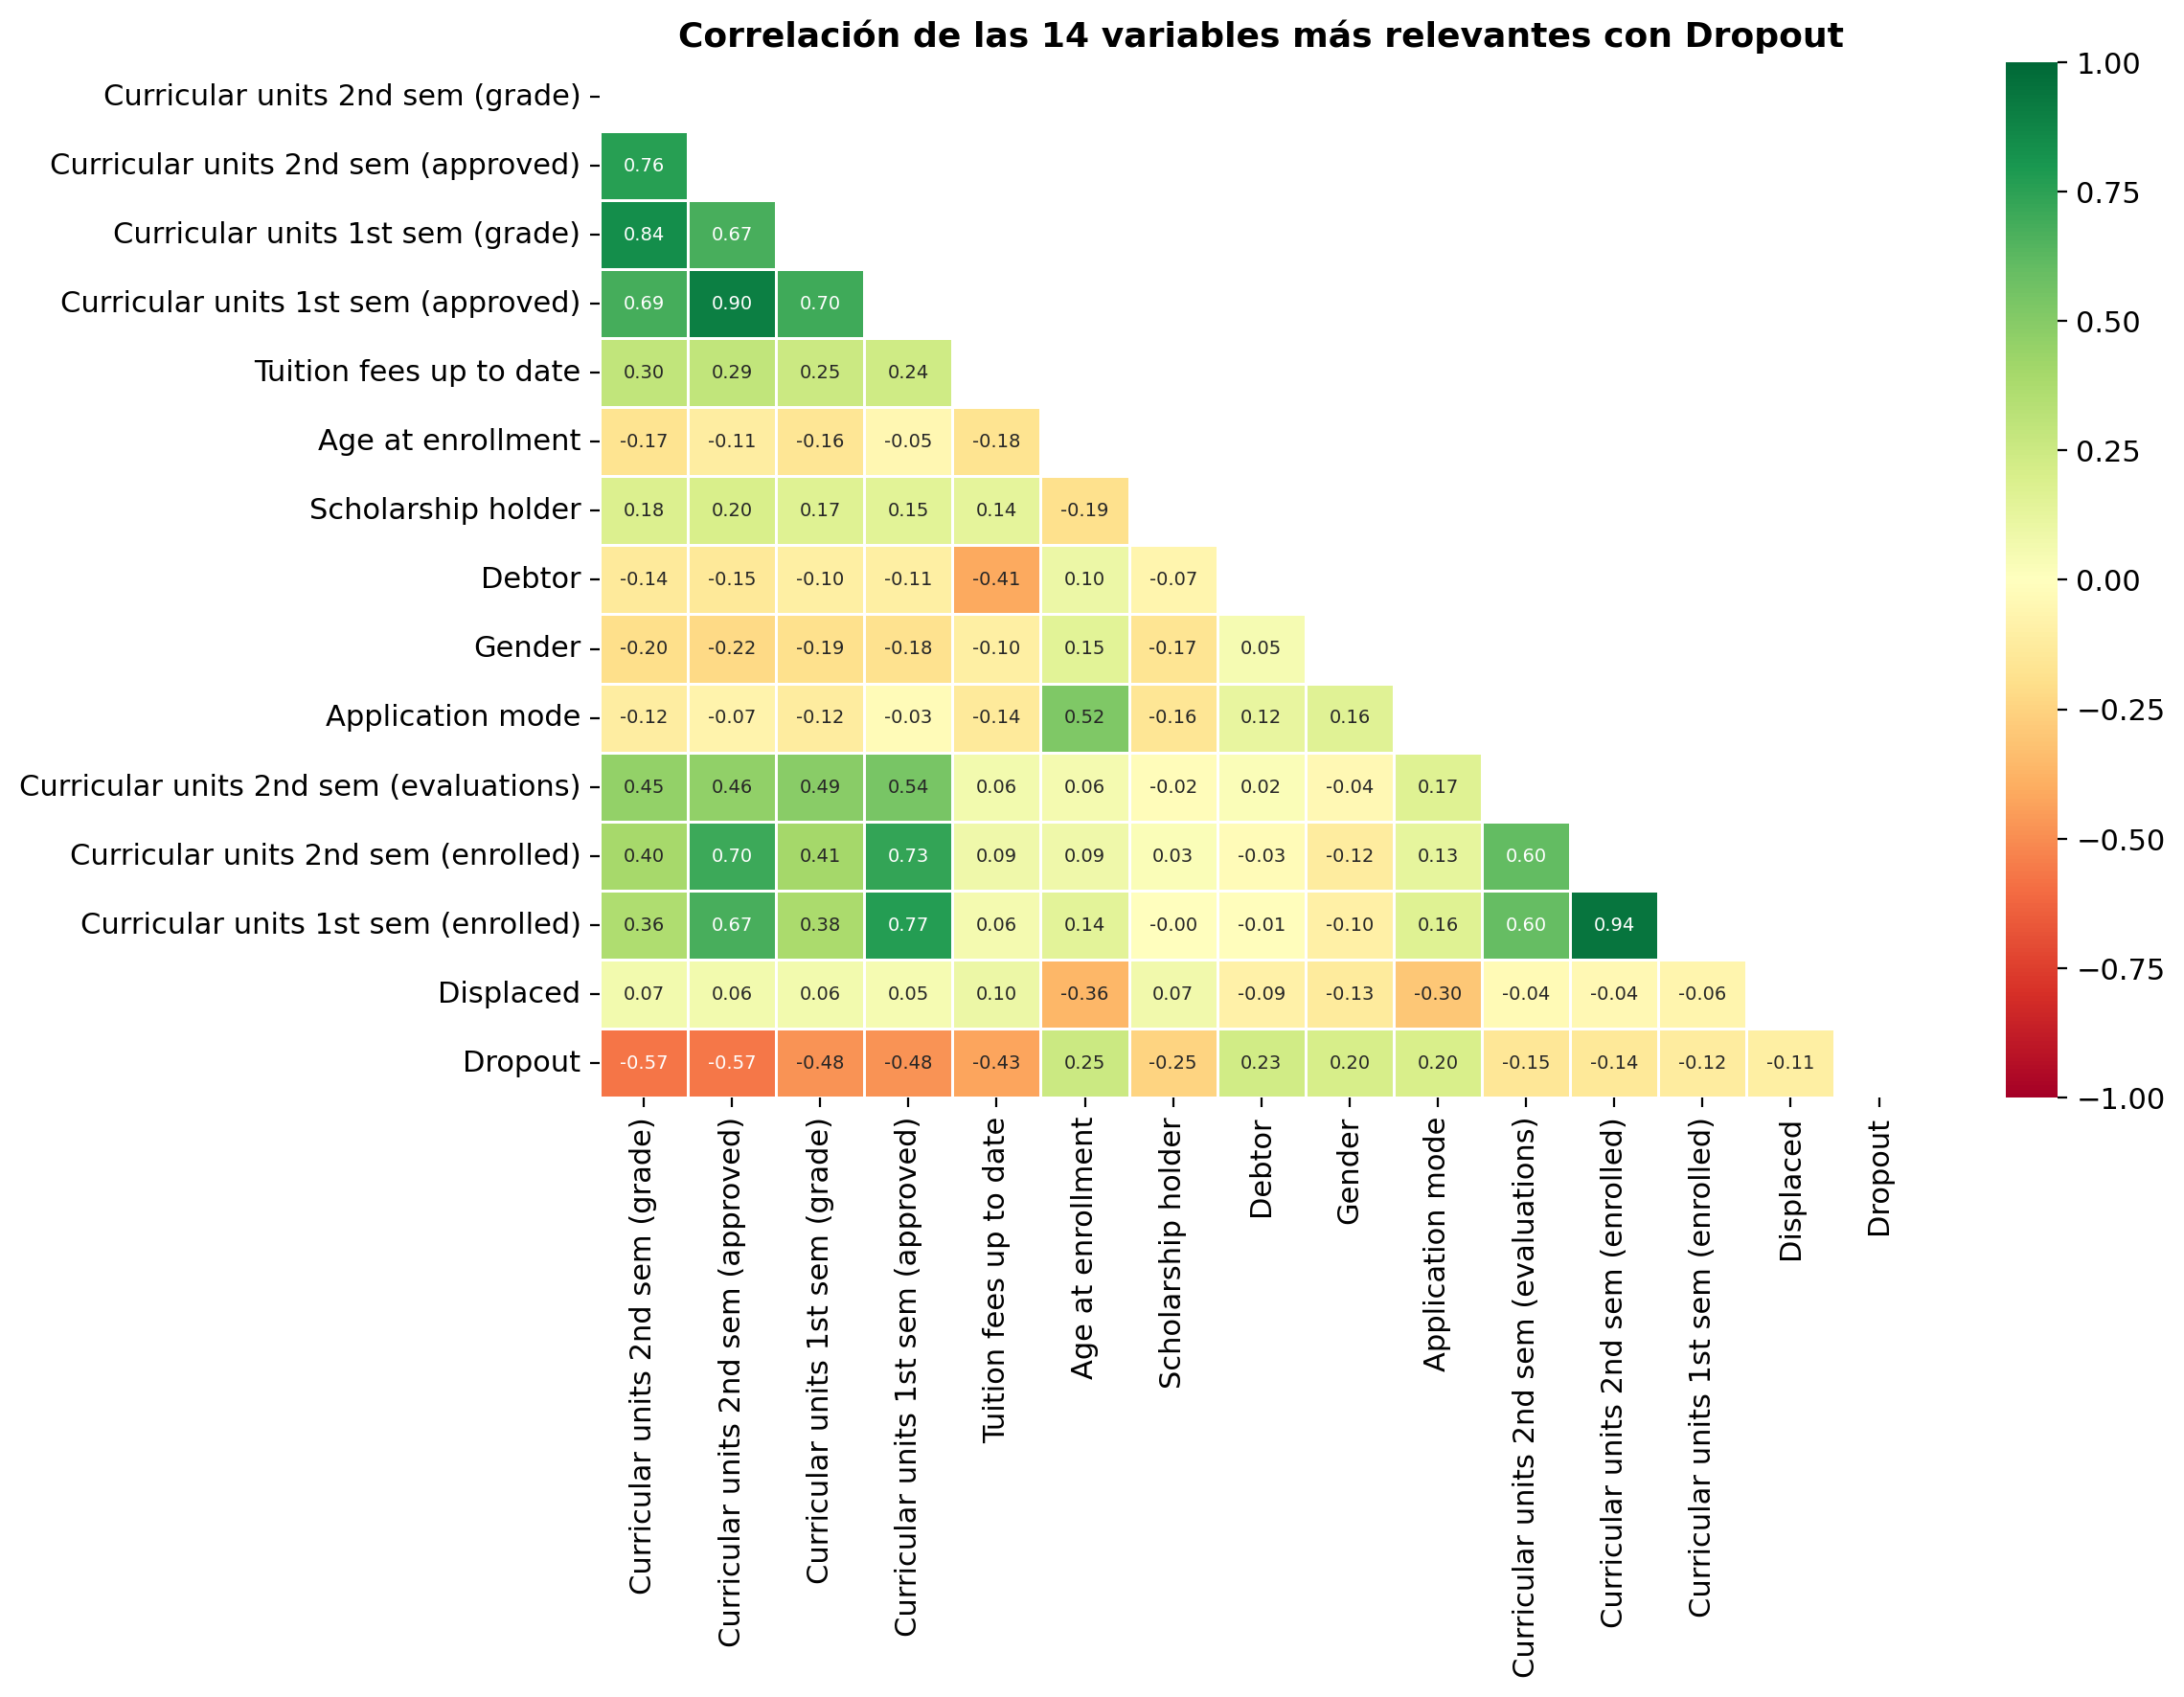
\includegraphics[width=0.85\textwidth]{figures/04_correlacion.png}
  \caption{Correlación de las 14 variables más relevantes con Dropout.
           Las unidades curriculares aprobadas dominan el ranking.}
  \label{fig:corr}
\end{figure}

% ============================================================
\section{Arquitectura del Sistema Multi-Agente}

El sistema combina un modelo ML clásico con un pipeline de cuatro agentes
orquestado en LangGraph~\cite{langgraph2024}. El patrón de ejecución es
\textit{fan-out} paralelo: los agentes EDA y RAG corren simultáneamente,
el agente ML actúa como barrera de sincronización (\textit{join}), y el
sintetizador produce el reporte final (Figura~\ref{fig:arq}).

\begin{figure}[H]
\centering
\begin{tikzpicture}[
    node distance=0.8cm and 1.8cm,
    box/.style={rectangle, draw, rounded corners=3pt,
                minimum width=2.2cm, minimum height=0.75cm,
                font=\small, align=center},
    arr/.style={->, >=Stealth, thick}
]
  \node[box, fill=gray!15]   (start) {START};
  \node[box, fill=blue!15,   above right=0.4cm and 1.6cm of start] (eda)  {Agente\\EDA};
  \node[box, fill=green!15,  below right=0.4cm and 1.6cm of start] (rag)  {Agente\\RAG};
  \node[box, fill=orange!15, right=4cm of start]                   (ml)   {Agente\\ML};
  \node[box, fill=red!15,    right=1.8cm of ml]                    (sint) {Agente\\Sintetizador};
  \node[box, fill=gray!15,   right=1.8cm of sint]                  (end)  {Reporte};
  \draw[arr] (start)--(eda); \draw[arr] (start)--(rag);
  \draw[arr] (eda)--(ml);    \draw[arr] (rag)--(ml);
  \draw[arr] (ml)--(sint);   \draw[arr] (sint)--(end);
\end{tikzpicture}
\caption{Arquitectura fan-out: EDA y RAG corren en paralelo; ML es la barrera de join.}
\label{fig:arq}
\end{figure}

Cada agente usa el LLM \texttt{llama-3.1-8b-instant} vía Groq~\cite{groq2024}
(\texttt{temperature}~$=0.2$) con prompts que inyectan datos reales del
sistema para minimizar alucinaciones. Los roles son:

\begin{table}[H]
  \centering\small
  \caption{Descripción de los cuatro agentes.}
  \label{tab:agentes}
  \begin{tabularx}{\textwidth}{lX}
    \toprule
    \textbf{Agente} & \textbf{Función} \\
    \midrule
    EDA          & Interpreta estadísticos reales del dataset e identifica variables de riesgo. \\
    RAG          & Recupera fragmentos de cinco papers desde ChromaDB y genera síntesis bibliográfica. \\
    ML           & Interpreta métricas del Random Forest y recomienda mejoras. \\
    Sintetizador & Integra los tres análisis en un reporte ejecutivo estructurado. \\
    \bottomrule
  \end{tabularx}
\end{table}

El módulo RAG~\cite{chromadb2023} indexa cinco documentos sobre deserción
(Tinto, factores académicos, socioeconómicos, enfoques ML y sistemas de
alerta temprana) en ChromaDB con embeddings \texttt{all-MiniLM-L6-v2}
(local, gratuito). En cada consulta se recuperan los cuatro fragmentos
más relevantes por similitud coseno.

% ============================================================
\section{Resultados}

\subsection{Comparación de modelos}

Se entrenaron tres modelos dentro de pipelines \texttt{scikit-learn} con
\texttt{StandardScaler} (ajustado solo en entrenamiento) y
\texttt{class\_weight='balanced'}. La Tabla~\ref{tab:modelos} resume las
métricas en validación; el Random Forest fue seleccionado por mayor AUC-ROC.

\begin{table}[H]
  \centering\small
  \caption{Comparación en validación. Baseline: DummyClassifier (clase mayoritaria).}
  \label{tab:modelos}
  \begin{tabular}{lccc}
    \toprule
    \textbf{Modelo} & \textbf{F1 (Dropout)} & \textbf{AUC-ROC} & \textbf{Avg Precision} \\
    \midrule
    Dummy (baseline)    & 0.0000 & 0.5000 & 0.3210 \\
    Logistic Regression & 0.7200 & 0.8734 & 0.8102 \\
    Gradient Boosting   & 0.7821 & 0.9289 & 0.8844 \\
    \textbf{Random Forest} & \textbf{0.7879} & \textbf{0.9335} & \textbf{0.8956} \\
    \bottomrule
  \end{tabular}
\end{table}

\subsection{Evaluación en test set}

El modelo ganador se evaluó una única vez en el test set. Las métricas
finales son: F1~$=0.7879$, AUC-ROC~$=0.9335$, Precisión~$=0.8525$,
Recall~$=0.7324$, Avg Precision~$=0.8956$. El AUC-ROC supera el rango
típico reportado en la literatura (0.85–0.93)~\cite{mduma2019}.
La Figura~\ref{fig:eval} muestra la matriz de confusión, la curva ROC
y la curva Precision-Recall; la Figura~\ref{fig:imp} presenta las
variables más predictivas.

\begin{figure}[H]
  \centering
  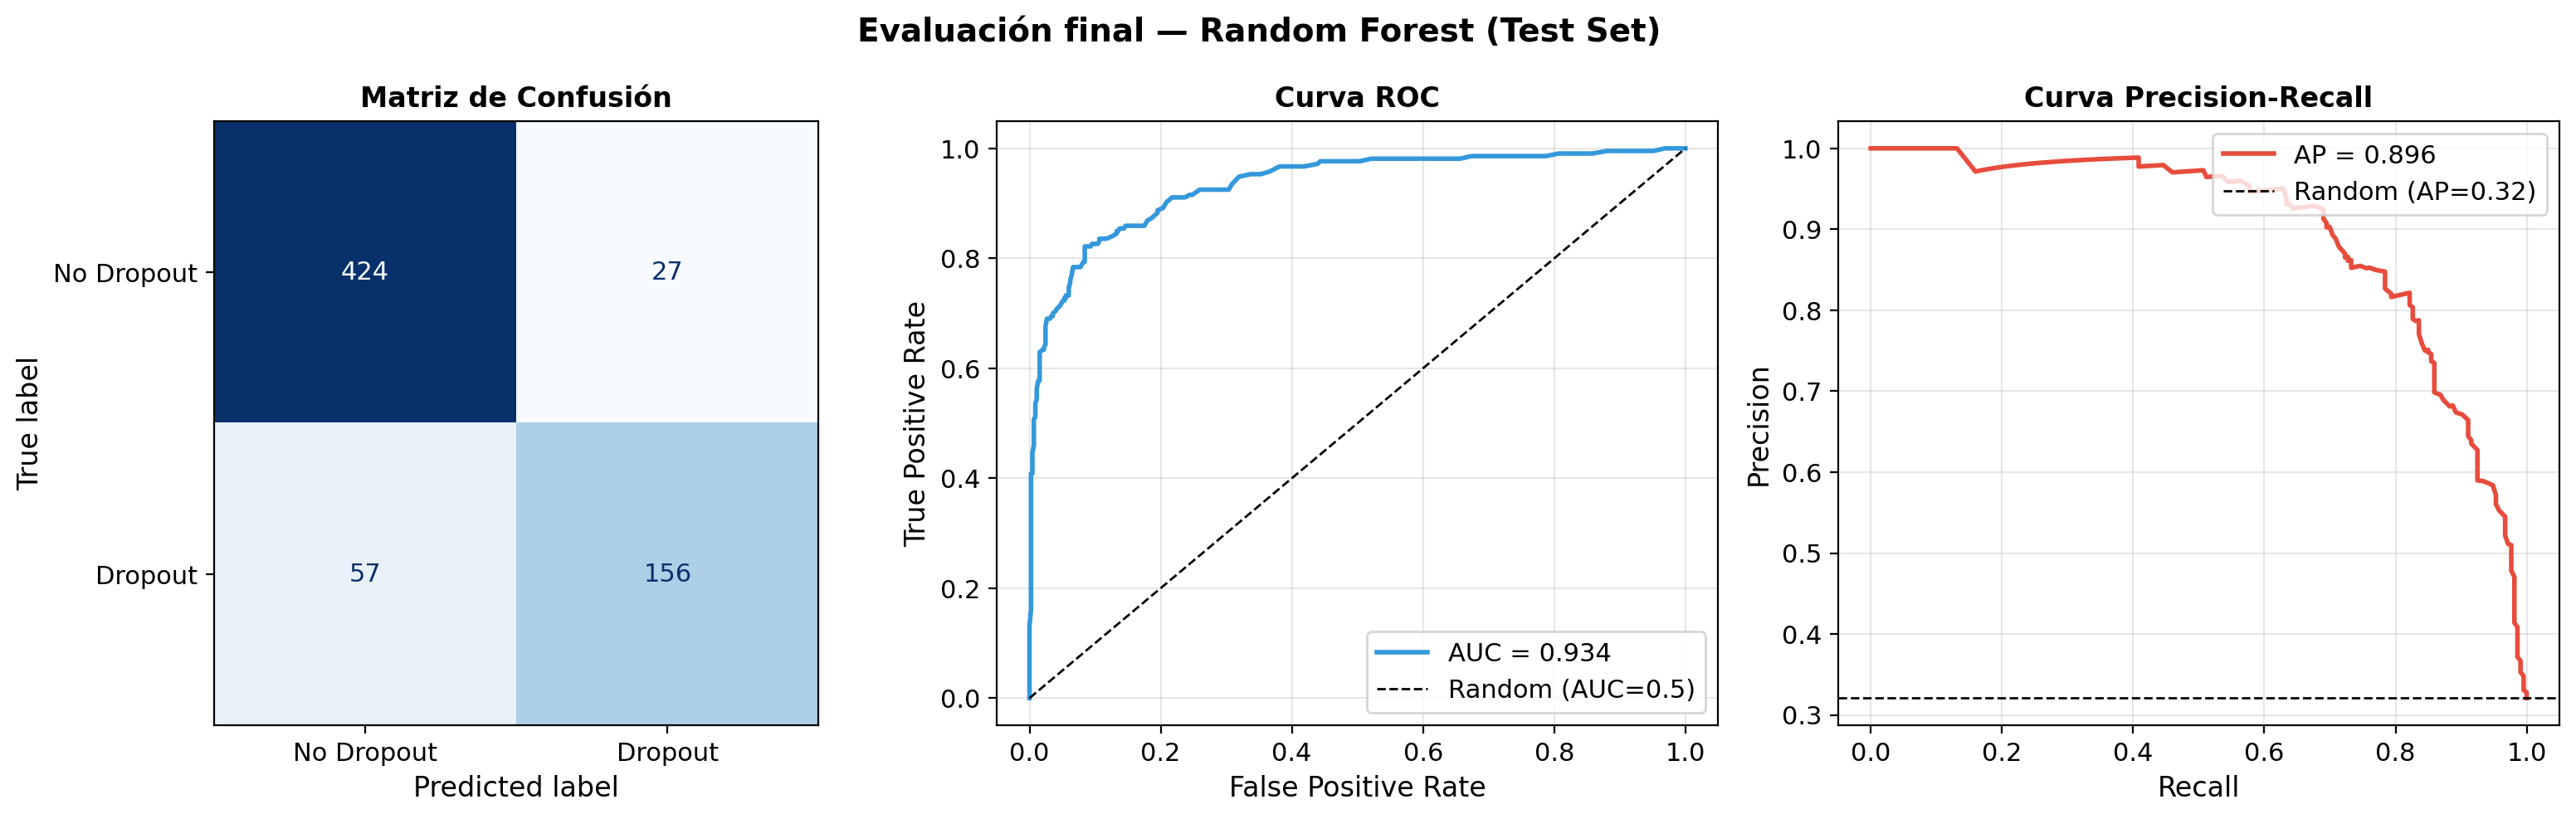
\includegraphics[width=\textwidth]{figures/08_evaluacion_final.png}
  \caption{Evaluación final en test set: matriz de confusión,
           curva ROC (AUC~$=0.9335$) y curva PR (AP~$=0.8956$).}
  \label{fig:eval}
\end{figure}

\begin{figure}[H]
  \centering
  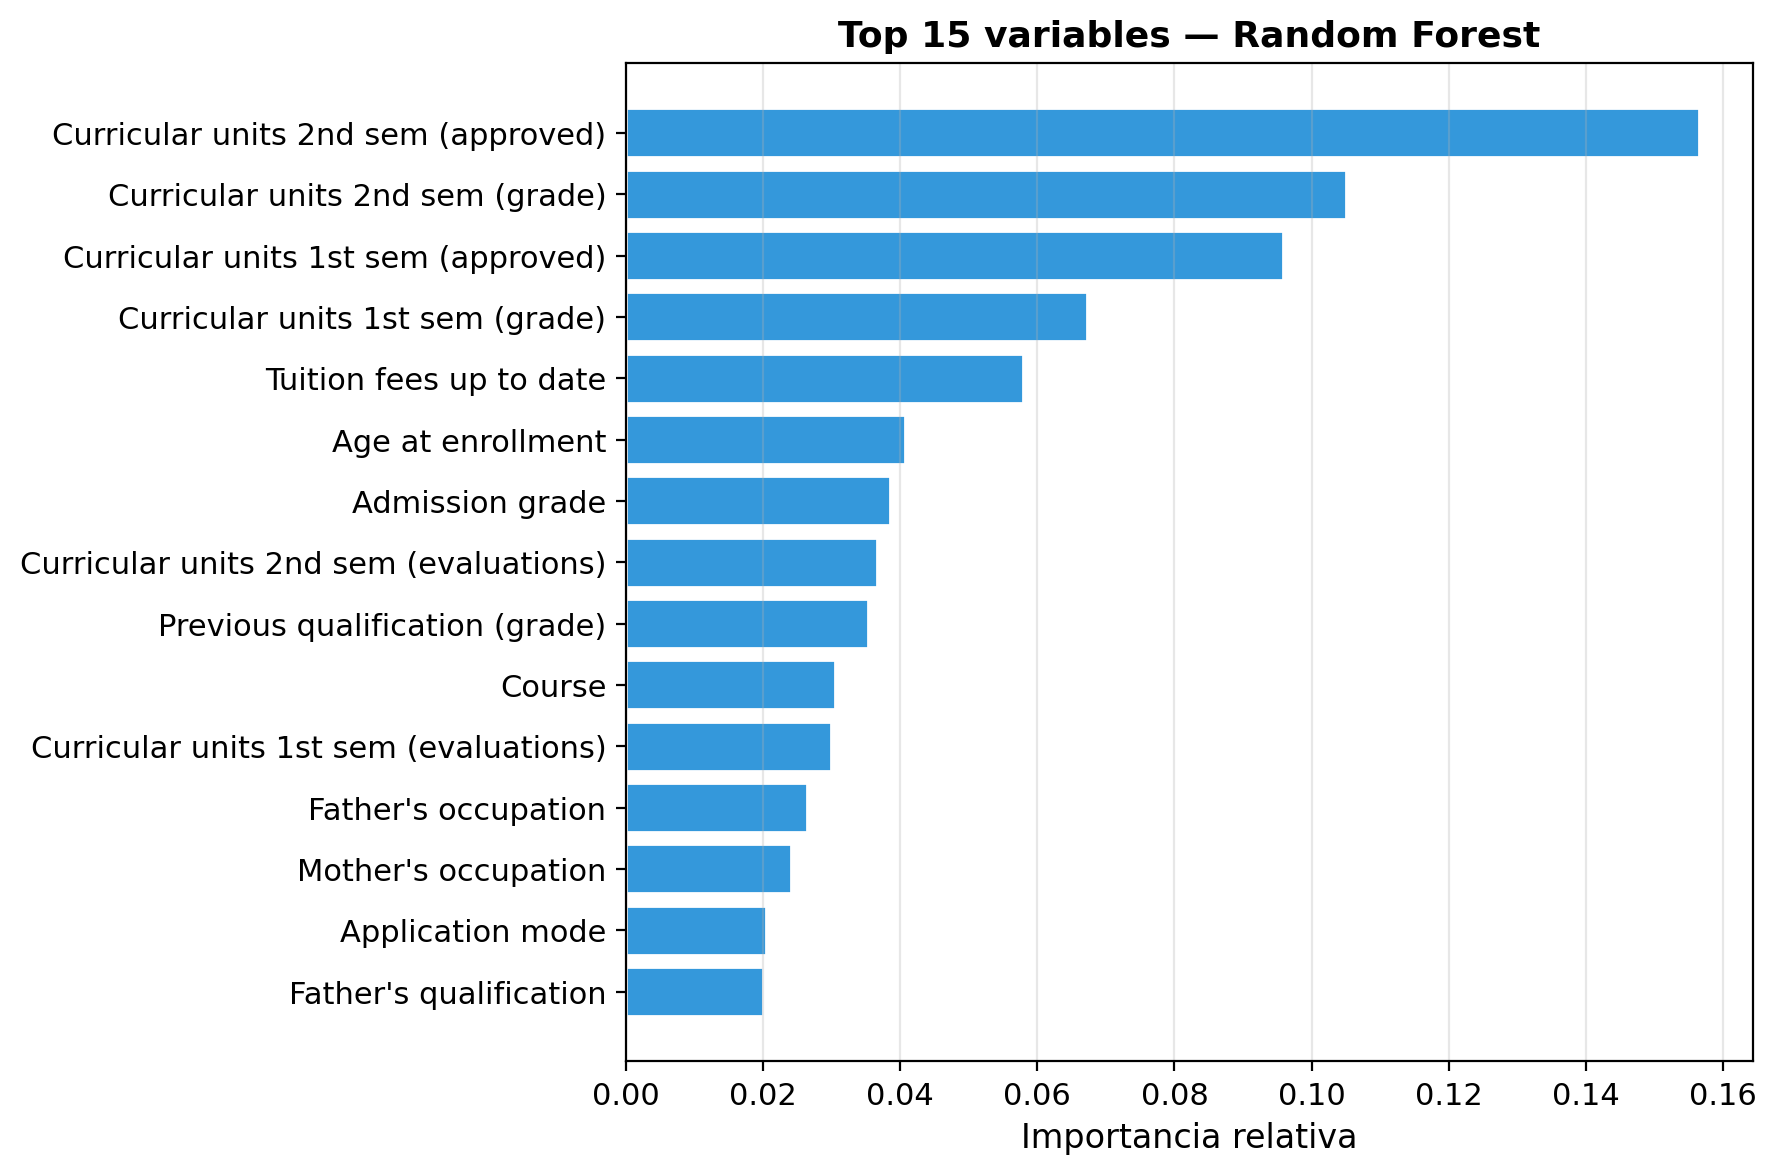
\includegraphics[width=0.78\textwidth]{figures/09_feature_importance.png}
  \caption{Top 15 variables según importancia del Random Forest.
           Las unidades aprobadas del 2.° semestre encabezan el ranking.}
  \label{fig:imp}
\end{figure}

\subsection{Evaluación del módulo RAG}

Se construyó un conjunto de diez preguntas con respuestas verificables
a partir del corpus y los datos reales del sistema (tasas de deserción,
variables predictivas, modelos reportados en la literatura). El sistema
respondió correctamente las diez preguntas (100\%), tal como muestra
la Figura~\ref{fig:rag}.

\begin{figure}[H]
  \centering
  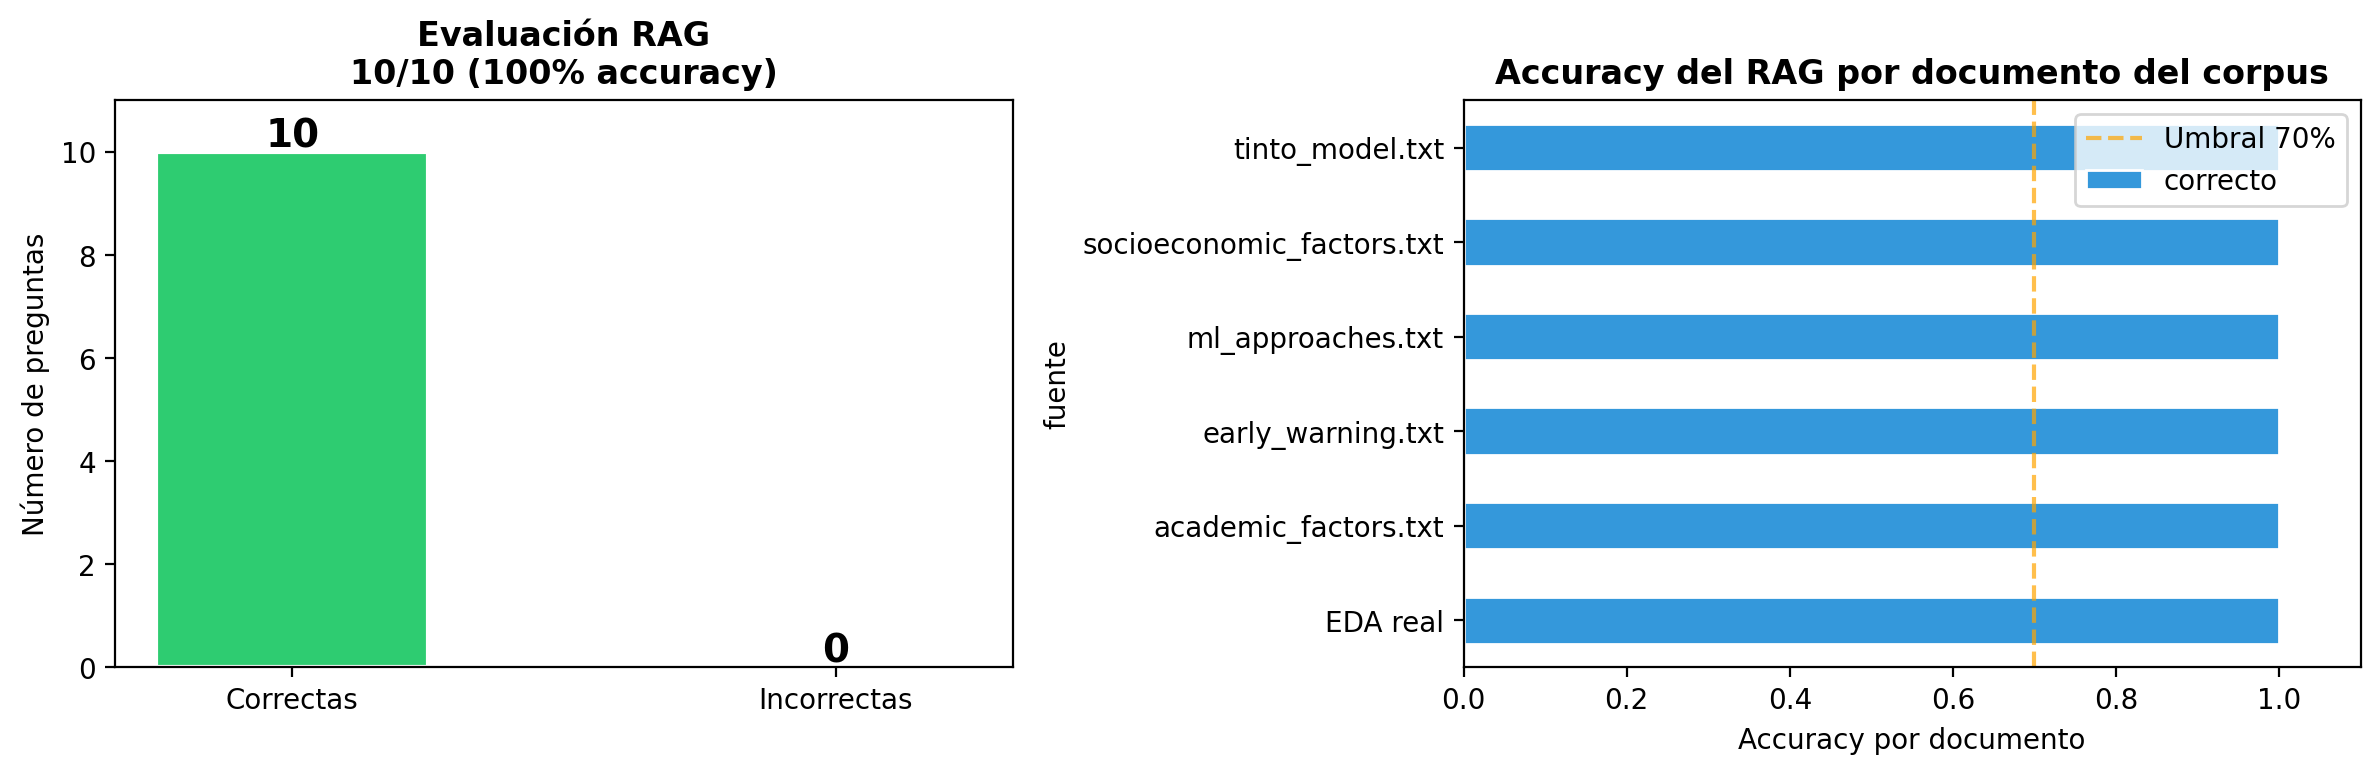
\includegraphics[width=0.68\textwidth]{figures/10_evaluacion_rag.png}
  \caption{Evaluación cuantitativa del RAG: 10/10 preguntas correctas.}
  \label{fig:rag}
\end{figure}

% ============================================================
\section{Conclusiones}

El sistema demuestra que es posible combinar ML clásico de alto rendimiento
(AUC-ROC~$=0.9335$) con agentes LLM que enriquecen el análisis con
literatura científica, todo con herramientas gratuitas y de código abierto.
El patrón \textit{fan-out} de LangGraph permite una arquitectura limpia y
extensible. El módulo RAG obtiene 100\% de exactitud en la evaluación,
validando la cobertura temática del corpus.

Como limitaciones: el conjunto de evaluación RAG es pequeño (10 preguntas)
y el dataset proviene de Portugal, lo que puede limitar su transferibilidad
a contextos latinoamericanos. Como trabajo futuro se propone incorporar
SMOTE para mejorar el recall (73.2\%), expandir el corpus con papers en
español, y desplegar la app en Streamlit Cloud o HuggingFace Spaces.

% ============================================================
\bibliographystyle{plain}
\bibliography{referencias}

\end{document}
